\chapter{Liouville and Contact Geometry for Dissipative Systems}
\label{chap:contact_mechanics} 
\section{Introduction}
\label{sec:contact_intro}
%\subsection{Historical perspective} 
The traditional theory of Hamiltonian mechanics based on symplectic manifolds does not include energy dissipation without an explicit time dependence. A famous example is the time-dependent Hamiltonian and Lagrangian functions modeling the linearly damped harmonic oscillator, which is commonly attributed to \citet{Caldirola1941} and \citet{Kanai1948}\footnote{We will hence refer to it as the Caldirola-Kanai Hamiltonian (or Lagrangian).}. 
These systems are nonautonomous, which is to say that the phenomenon of dissipation is essentially treated to be \emph{exogeneous} from the perspective of the system.  

To the engineer, this does not seem natural at all. Every physical system, be it mechanical, electrical, economic, or otherwise, includes dissipative elements in some shape or form. These elements are inherent to the system: exogenous effects are typically reserved for externally controlled inputs or disturbances. Hence, from an engineering point of view, we seek to include the dissipative elements as phenomena that are \emph{endogeneous} to the system itself.

Some efforts have been made in the past to resolve this issue by extending the Hamiltonian formalism: the celebrated report by \citet{Dekker1981} provides an excellent overview of the advances in this field. Roughly speaking, three approaches exist:
\begin{itemize}
    \item The \emph{Bateman approach}, doubles the number of degrees of freedom in the system to create a `mirror system' that runs in the opposite time direction \cite{Bateman1931}. In the overall system the irreversible (i.e. dependent on the direction of time) effects, cancel out due to the two time directions, which is why it admits a symplectic structure.
    \item The family of \emph{complex dissipative Hamiltonians} proposed in various forms by \citet{Bopp1974}, \citet{Dekker1975}, \citet{Dedene1980}, \citet{Rajeev2007}, and more recently, \citet{Hutters2020} in the research group of the author. Originally, this method was developed to facilitate the quantization of dissipative mechanics for applications in quantum mechanics. The relation of the work in this thesis with the complex dissipative Hamiltonians is given in \cref{ssec:complex_ham}.
    \item Some purely \emph{mathematical Hamiltonians} have been devised as well, e.g. by \citet{Havas1957} solving the so-called Helmholtz conditions. These Hamiltonians produce the correct equations of motion but bear no connection to the energy in the system.
\end{itemize}
Although all of these methods work, they have some limitations for practical applications. The Bateman approach results in a system with twice the dimensions, but most (at least half) of these are redundant. This is because dissipation is in essence a first-order effect: as will be shown in this chapter, at most one additional dimension is required to model the dissipation. The complex Hamiltonians are mathematically elegant but lack physical interpretation of the canonical  coordinates and the Hamiltonian function. Finally, the mathematical Hamiltonians do not offer insights from a physical standpoint. Furthermore, they rely on singularities of the Hamiltonian function to circumvent the inevitable limitations imposed by de Rham's theorem (this point is discussed in greater detail later in \cref{sec:liouville}).

In addition, we remark that it is common practice in engineering applications to include the \emph{Rayleigh damping function} in the Lagrangian function \cite{Goldstein2011} to represent linearly damped elements. Although this damping function produces the correct equations of motion for linear damping, it does not conform to the deeper symplectic structure underlying Hamiltonian (and also Lagrangian) mechanics. Hence, we consider this an \emph{ad hoc} method, and we will not be further concerned with it in this thesis.

The purpose of this chapter is to propose a different framework that is both mathematically elegant \emph{and} physically interpretable, to make it suitable for practical applications. Instead of trying to fit the dissipation into the symplectic framework, we propose that \emph{contact manifolds} (instead of symplectic manifolds) are the natural setting for problems that include dissipation. Contact manifolds are necessarily odd-dimensional: next to the canonical pairs of positions of momenta, an extra coordinate is included that absorbs the dissipated energy. The Hamiltonian formalism can be extended from symplectic manifolds to contact manifolds as well. We will use this \emph{contact Hamiltonian formalism} to describe dissipative mechanical systems.

This chapter takes two different paths to arrive at a single contact Hamiltonian representation of the damped harmonic oscillator, which serves as an exemplary dissipative system. These two paths are based on two parallel mathematical representations of a contact manifold: one is the contact structure itself, while the other is its \emph{symplectification}. This is a procedure to cast the contact Hamiltonian system on a symplectic manifold with an additional \emph{Liouville structure}. This procedure goes at the expense of yet another dimension added to the manifold, making it even-dimensional again.

Firstly, in \cref{sec:thermodynamics}, we use the principles of thermodynamics to derive the contact Hamiltonian representation of the damped harmonic oscillator. Secondly, in \cref{sec:liouville}, we look at the symplectification of the manifold and derive an equivalent symplectified Hamiltonian system argued motivated by the form of the Caldirola-Kanai Hamiltonian.

We then proceed by transforming the contact Hamiltonian representation of the damped harmonic oscillator to the contact Lagrangian representation in \cref{sec:lagrangian}. Finally, \cref{sec:generalization} shows how the same principles can be used to model more complicated mechanical systems, including those with exogenous inputs.
%<symbol: \gamma> <expl: Damping coefficient> <tags: greek, mech>

For the reader unfamiliar with contact geometry and contact Hamiltonian systems, a concise introduction to contact geometry and contact Hamiltonian systems is given in \cref{app:contact_geometry}. A more extensive overview is given by \citet{Geiges2008} and \citet{Libermann1987}.

%% THERMODYNAMIC REASONING
\section{Contact structure from thermodynamics}
\label{sec:thermodynamics}
It has already been argued in the past by several authors that contact geometry is the natural framework for thermodynamics by i.a. \citet{Arnold1991,Arnold1989a,Arnold1989,Arnold1989b}, \citet{Bamberg1988}, \citet{Burke1985} and \citet{Hermann1973}, ultimately leading back to the seminal work of \citet{Gibbs1873}. It is a testament to the brilliance of Gibbs' work that he managed to recognize and describe the correct geometric framework well before the required mathematical infrastructure even came to invention \cite{Wightman1979}. 
In recent years, the contact Hamiltonian formalism has been succesfully applied to thermodynamic theory by e.g. \citet{Mrugala1991,Mrugala2000,Mrugala1984,Mrugala1985,Mrugala1993,Mrugala1996}, \citet{Balian2001}, \citet{VanderSchaft2021a}, \citet{Bravetti2015}, and \citet{Simoes2020}. Interestingly, the applicability of the contact Hamiltonian formalism for mechanical systems with dissipation has been described already by \citet{Bravetti2017}, in particular for the damped harmonic oscillator. However, we argue that his argument is purely mathematical (that is, it produces the correct equations of motion) without interpretation. Indeed, the case is made here that it is also essential to recognize the Hamiltonian function as the total energy in the system, even for dissipative systems; this point is also not addressed by \citeauthor{Bravetti2017}. Precisely these insights lead allow us to use the theory from thermodynamics to find a constructive approach to dissipative systems.

The contact structure in thermodynamics arises as a consequence of the First Law, which says that the change in internal energy of the system is equal to the difference between the heat added \emph{to} the system and the work performed \emph{by} the system. Formally, this is stated as
\begin{equation}
    \dd{U} = \eta - \beta,
    \label{eq:thermo_first_law}
\end{equation}
where $U$ is the internal energy of the system, $\eta$ the heat added to the system and $\beta$ the work done by the system on its environment \cite{Bamberg1988,Frankel2012}. Both $\eta$ and $\beta$ are 1-forms that are not exact.  This is why it makes no sense (in the context of exterior systems) to denote them by \dj and $\dd{W}$, or worse, using the `inexact' surrogate notation $\text{đ}$ or $\delta$. The essence of the First Law really is that the difference of the heat and work forms is \emph{closed}. Locally, it can then be written as the gradient of a function, called the \emph{internal energy} $U$ of the system. As a result, the form 
$$ \alpha = \dd{U} - \eta + \beta $$
should pull back to zero over the `allowable' states of the systems.

Classical thermodynamics is usually geared towards systems containing expanding gases or chemical mixtures, and not purely mechanical systems. This is why in the next section is first applied to a simple thermodynamic system to elucidate the significance of contact geometry in thermodynamics, after which \cref{ssec:thermo_dho} is concerned with the application to purely mechanical systems.

\subsection{Contact structures in thermodynamics} 
%<symbol: P> <expl: Pressure> <tags: letter, thermo>
%<symbol: V> <expl: Volume> <tags: letter, thermo>
%<symbol: T> <expl: Temperature> <tags: letter, thermo>
%<symbol: R> <expl: Universal gas constant> <tags: letter, thermo>
%<symbol: n> <expl: Amount of substance> <tags: letter, thermo>
The thermodynamic state of a system is given by a collection of thermodynamic state variables (or `properties'). For example, for an ideal gas in a piston, we may consider its volume $V$, temperature $T$ and pressure $P$. However, we also know, that for an ideal gas, the following relation must hold:
\begin{equation}
    PV = nRT,
    \label{eq:ideal_gas}
\end{equation}
with $n$ is the amount of substance (measured in \si{\mole}), and $R = \SI{8.314}{\joule \per \mole \per \kelvin}$ is the ideal gas constant.  Hence, for a constant number of moles the actual state of the system is dictated only by two state properties, for the ideal gas law allows us to find the other if two out of three are given. The states of the system that are thermodynamically meaningful therefore live on a \emph{two-dimensional submanifold} of $\real^3$. Any selection of two state properties may serve as coordinates for this submanifold. However, due to this ambiguity, it is usually more convenient to consider the larger three-dimensional manifold together with the constraint  \cite{Balian2001, Giancoli2014}.

Now, if we are allowed to add heat to the gas in the piston, or we use its expansion to perform work on the environment, \cref{eq:ideal_gas} will not suffice because it does not contain \emph{all} the thermodynamic information of the system. The additional information is supplied (for example) in terms of the entropy $S$ in the system. A \emph{fundamental thermodynamic relation}, expresses a thermodynamic potential, such as the internal energy $U$, in terms of the extensive variables in the system. For the ideal gas, the fundamental relation is of the form $U = U(S, V)$, for the entropy $S$ and the volume $V$ are the extensive state properties of the system. The choice of the internal energy as the thermodynamic potential is certainly not unique; we may also invert the relation in favor of the entropy or use other potentials obtained through a Legendre transform, such as the Gibbs free energy, Helmholtz free energy, enthalpy etc. In particular, we refer to the specification of a system in terms of internal energy as the \emph{energy representation}, and to a specification in terms of entropy as the \emph{entropy representation} \cite{VanderSchaft2021a}.

In the spirit of the preceding discussion, we now consider a five-dimensional space to describe the complete thermodynamic state of the system. Coordinates for this space are the internal energy and entropy in addition to the pressure, volume and temperature considered earlier. This space is referred to as the \emph{thermodynamic phase space} $M$. Again, we are not to choose these variables completely independent from each other, since they are subject to constraints. The First Law of thermodynamics states that
$$ \dd{U} = \eta - \beta, $$
%<symbol: U> <expl: Internal energy> <tags: letter, thermo>
%<symbol: \eta> <expl: Heat 1-form> <tags: greek, thermo>
%<symbol: \beta> <expl: Work 1-form> <tags: greek, thermo>
%<symbol: S> <expl: Entropy> <tags: letter, thermo>
where we have that $ \beta = P\dd{V} $ and, according to the Second Law of Thermodynamics, $ \eta = T\dd{S} $. As such, the First Law states that the form
\begin{equation} 
    \alpha = \dd{U} - T\dd{S} + P\dd{V}
    \label{eq:gibbs_relation}
\end{equation}
should pull back to zero on the allowable states. This relation is known as Gibbs' fundamental relation. By definition --- given that the internal energy is a function of the extensive state variables ---  we furthermore have that
$$ \dd{U} \coloneq \pdv{U}{V}\dd{V} + \pdv{U}{S}\dd{S}.$$
As such, the condition that $\alpha = 0$ defines an two-dimensional submanifold of the larger five-dimensional space for which we have:
\begin{equation}
    T = \pdv{U}{S} \qquad P = -\pdv{U}{V}. 
\end{equation}
The form $\alpha$ given by Gibbs' relation is a contact form on the thermodynamic phase space, since
$$ \wedgep{\alpha}{(\dd{\alpha})^2} = 2\,\dd{U}\wedgep{\wedgep{\dd{S}}{\dd{T}}}{\wedgep{\dd{P}}{\dd{V}}}, $$
which is a top form on the thermodynamic phase space.\footnote
{
    Because 
    \begin{equation*} 
        \begin{split}
            (\dd{\alpha})^2 &= (\wedgep{\dd{S}}{\dd{T}} + \wedgep{\dd{P}}{\dd{V}})^2 \\
                            &= \wedgep{\wedgep{\dd{S}}{\dd{T}}}{\wedgep{\dd{P}}{\dd{V}}} + \wedgep{\wedgep{\dd{P}}{\dd{V}}}{\wedgep{\dd{S}}{\dd{T}}} \\
                            &= 2\wedgep{\wedgep{\dd{S}}{\dd{T}}}{\wedgep{\dd{P}}{\dd{V}}} \\
        \end{split}
    \end{equation*}
    since the permutation $ (S, T, P, V) \mapsto (P, V, S, T) $ is even.
}
Manifolds on which $\alpha$ pulls back to zero are called integral submanifold. Due to the nondegeneracy of the contact form, these submanifolds are of dimension 2; these maximal integral submanifolds are called \emph{Legendre submanifolds}. Clearly, Legendre submanifolds play a pivotable role in this framework because they define the thermodynamically allowable states (\citet{Balian2001} call them \emph{thermodynamic manifolds}).

\subsection{Thermodynamics of the damped oscillator}
\label{ssec:thermo_dho}
\paragraph{Extensive and intensive variables} In contrast to thermodynamics, there does not seem to be an unequivocal distinction between extensive and intensive variables for mechanical systems. Although it is not strictly a problem from a mathematical standpoint, the internal energy is usually stated to be a function of the extensive state properties. To incorporate kinetic energy, the internal energy function should be a function of either momentum or velocity: the former is used necessarily used in the Hamiltonian formalism. However, it is not so clear whether momentum is intensive rather than extensive. For example, \citet{Franksen1969} argues that momentum should be considered as extensive, for mass is related to the `size' of the system. 

\paragraph{Contact structure} For the damped harmonic oscillator, we consider the \emph{overall} system to be completely isolated: that is, there is no energy in the form of work or heat added to the system (for we consider the damper part of the system itself). As a result, the First Law simply states that
$$ \dd{U} = 0. $$
The internal energy of the mass-spring-damper system is a function of the position $q$ of the mass, the momentum $p$ of the mass and the entropy $S$ generated by the damper, i.e.
$$ U = U(q, p, S). $$
In this system, internal energy can be stored either in the form of macroscopic kinetic energy in the mass, potential energy in the spring and as microscopic kinetic energy of the damper fluid. Please note that the damper fluid is rather loosely defined: it can also encompass a body of surrounding air, or anything to which we may attach the conceptual picture of a `heat bath' that absorbs the dissipated energy in the form of heat. Furthermore, we assume that the heat bath is the only part of the system that can store entropy. Let uw now decompose the system into two subsystems: first, the mass-spring system storing the mechanical energy. 
The total internal energy then becomes:
$$ U(q, p, S) = U_1(q, p) + U_2(S) = \frac{p^2}{2m} + \frac{1}{2}kq^2 + U_2(S). $$
If specific assumptions are made about the nature of the heat bath, an explicit expression for $U_2$ may be found as well (e.g. an ideal gas), but we will leave this possibility open for now. The decomposition into the two subsystems is illustrated by \cref{fig:oscillator_thermo}.
\begin{figure}[ht!]
    \centering
    \begin{tikzpicture}[every node/.style={outer sep=0pt,thick}, scale=2]
    \tikzstyle{spring}=[thick,decorate,decoration={zigzag,pre length=1cm,post length=1cm,segment length=12, amplitude=0.2cm}]
    \tikzstyle{damper}=[thick,decoration={markings,  
      mark connection node=dmp,
      mark=at position 0.4 with 
      {
        \node (dmp) [thick,inner sep=0pt,transform shape,rotate=-90,minimum width=30pt,minimum height=30pt,draw=none] {};
        \draw [thick, {Bar[width=6pt]}-{Bar[width=6pt]}] ($(dmp.north east)+(16pt,13pt)$) -- ($(dmp.north east)+(16pt,0)$) -- (dmp.south east) -- (dmp.south west) -- ($(dmp.north west)+(16pt,0)$) -- ($(dmp.north west)+(16pt,-13pt)$);
        \draw [very thick] ($(dmp.north)+(0pt,-12pt)$) -- ($(dmp.north)+(0pt,12pt)$);
      }
    }, decorate]
    
    \tikzstyle{ground}=[thick,fill,pattern=north east lines,draw=none,minimum width=0.75cm]
    
    \node at (-2.7, -0.9) (leftcorner) {};
    \node at (0.7, 0.9) (rightcorner) {};
    \node at (-2.7, 0.05) (leftsplit) {};
    \node at (-1, -0.9) (rightsplit) {};
    
    %\draw[] (-2.7, 0.05) -| (-1, -0.9); 
    
    \draw[thick] (-2.7, -0.9) rectangle (0.7, 0.9); 
    \filldraw[fill=accent2!30] ($(leftsplit) +(1.5pt,-0.75pt)$) rectangle ($(rightsplit) +(-0.75 pt,1.5pt)$);
    \filldraw[fill=accent1!30] ($(rightsplit) +(0.75 pt,1.5pt)$) -| ($(rightcorner) +(-1.5pt,-1.5pt)$) -| ($(leftsplit) +(1.5pt,0.75 pt)$) -| cycle;
    
    \node (M) [draw,minimum width=2cm, minimum height=3cm] {};
    
    \node (ground) [thick,anchor=north,yshift=-0.25cm,minimum width=1.5cm] at (M.south) {};
    %\draw (ground.north east) -- (ground.north west);
    %\draw [thick] (M.south west) ++ (0.2cm,-0.125cm) circle (0.125cm)  (M.south east) ++ (-0.2cm,-0.125cm) circle (0.125cm);
    
    \node (wall) [ground,thick, rotate=-90, minimum width=4cm,yshift=-6cm] {};
    \draw (wall.north east) -- (wall.north west);
    
    \draw [spring] (wall.172) -- ($(M.north west)!(wall.172)!(M.south west)$) node[pos=0.5,anchor=south, outer sep=8pt] {};
    \draw [damper] (wall.8) -- ($(M.north west)!(wall.8)!(M.south west)$) node[pos=0.5,anchor=north, outer sep=20pt] {};
    
    \draw[{Circle[open,length=2pt]}-] (-0.7, 0.6) -- (-0.7, 1.5) node[draw, thin, inner sep = 3mm, anchor=south] {\small{$\displaystyle E = \frac{p^2}{2m} + \frac{1}{2}kq^2$}}; 
    \draw[{Circle[open,length=2pt]}-] (-1.2, -0.6) -- (-1.2, -1.3) node[draw, thin, inner sep = 3mm, anchor=north] {\small{$U$}}; 
    
\end{tikzpicture}

    \caption{Blabla}
    \label{fig:oscillator_thermo}
\end{figure}
Because there is transfer of energy within the system, we must apply the First Law these two subsystems separately as well. We know that the first subsystem performs work on the damper fluid, which manifests itself as heat added to the second subsystem. We therefore have
\begin{equation}
    \begin{split}
        \dd{U}_1 &= -\beta_1, \\
        \pdv{U_1}{p}\dd{p} + \pdv{U_1}{q}\dd{q} &= -\beta_1, \\[0.2cm]
        \dd{U}_2 &= \eta_2, \\
        \pdv{U_2}{S}\dd{S} &= \eta_2, \\
    \end{split}
\end{equation}
where $\beta_1$ is the (differential) work done by the mechanical subsystem and $\eta_2$ is the (differential) heat added to the second subsystem. From the preceding discussions we have that, because the total system is isolated, that $ \beta_1 = \eta_2 $; i.e. all the work done by the damper enters the fluid as heat. For a linearly damped system, the work form is equal to 
$$ \beta \coloneq \gamma p \dd{q}. $$
As such, the contact form dictated by the First Law on the three-dimensional manifold constituted by the internal energy of the heat bath $U_2$, the momentum of the mass $p$ and the position of the mass $q$
\begin{equation}
    \alpha_2 = \dd{U}_2 - \gamma p \dd{q};
    \label{eq:dho_contact_form_thermo}
\end{equation}
or equivalently
\begin{equation*}
    \alpha_1 = -\dd{U}_1 + \gamma p \dd{q}.
\end{equation*}

Given this contact structure, we are now to find the contact Hamiltonian function to complete the picture of the contact Hamiltonian system. A contact Hamiltonian system is a triple $(M, \alpha, H)$, where $M$ is a manifold, $\alpha$ is a contact structure on the manifold and $H$ is the Hamiltonian function that generates the dynamics. Just like in the conservative symplectic case the contact structure provides a mapping between the functions on the manifold and the `contact Hamiltonian vector fields' on that manifold. This mapping is discussed in detail in \cref{sec:contact_ham_systems}. The trick is to decompose the Hamiltonian vector field into a horizontal and a vertical vector field; that is
$$ \tbundle{M} = \ker \alpha \oplus \ker \dd{\alpha},$$
where the vertical component is in the kernel of $ \dd{\alpha}$, and the horizontal vector field in the kernel of $ \alpha $. The Hamiltonian vector field is then 
$$ X_H = X_H^\text{ver} + X_H^\text{hor.}, $$
with $X_H^\text{ver} \in \ker \dd{\alpha}$ and $X_H^\text{hor} \in \ker \alpha$.
Furthermore, we impose two conditions on the Hamiltonian vector field $X_H$ associated to the Hamiltonian $H$. First, we have that $ H = = \intpr{X_H}{\alpha} $. The second condition is that $\lied{X_H}\alpha = s \alpha $ with $s$ some function; which is to say that $X_H$ is an infinitesimal contact transformation. 

The vertical part of the vector field is easy to find based on the first condition, and is equal to
$$ X_H^\text{ver} = -H R_\alpha. $$
However, for reasons that will become later, the horizontal part is of our prime interest. This part is obtained using the second condition, which is equivalent to
\begin{equation}
    \intpr{X_H^\text{hor}}{\dd{\alpha}} = \dd{H} - (\intpr{R_\alpha}{\dd{H}}) \alpha 
    \label{eq:hor_vfield_condition}
\end{equation}

Now, recall that for a purely symplectic (i.e. energy-conserving) Hamiltonian system, the relation between the Hamiltonian vector field and the Hamiltonian is given by (see \cref{app:symplectic_geometry} for details) 
$$ \dd{H} = \intpr{X_H}{\omega}, $$
where $\omega$ is the symplectic form, in this case $\omega = \wedgep{\dd{q}}{\dd{p}}$. By definition, we have that the form $\dd{\alpha}$ is also symplectic; it is easily checked that we have that $\dd{\alpha} = \omega$. The relation above then becomes 
$$ \dd{U_1} = \intpr{X_{U_1}}{\dd{\alpha}} - \text{dissipation}, $$
since the Hamiltonian of this system will be purely given by the mechanical energy in the absence of a dissipative element. Naturally, the system at issue is \emph{not} conservative, which is why we cannot expect the symplectic relation to hold. Instead, we expect to see a defect that measures the deviation from the ideal symplectic situation in the form of an extra term appearing in the above relation, representing the `leakage' of mechanical energy from the system. This is indeed what is obsered from \cref{eq:hor_vfield_condition}: the second term appearing on the right represents the dissipative action. Based on the expression for the contact form in \cref{eq:dho_contact_form_thermo}, we have
\begin{equation} 
    \begin{split}
        \intpr{X_H^\text{hor}}{\dd{\alpha}} &= \dd{H}  - \pdv{H}{U_2}U_2 + \pdv{H}{U_2}\gamma p\dd{q} \\
        \intpr{X_H^\text{hor}}{\dd{\alpha}} - \pdv{H}{U_2}\gamma p\dd{q} &= \dd{H}  - \pdv{H}{U_2}\dd{U_2}
    \end{split}
\end{equation}
As such, we recover the expected expression stated above \emph{if} $\dd{H} - \pdv{H}{U_2}\dd{U_2} = \dd{U_1}$. Let us make the convenient choice that $\pdv{H}{U_2} = 1$, which means that 
$$ H = U = U_1 + U_2, $$
at up to an arbitrary additive constant, which we choose to be zero. Hence, the \emph{contact Hamiltonian is equal to the total internal energy in the system}.

The contact Hamiltonian vector field then becomes  
$$ \text{derive equations of motion} $$

The vertical vector field is proportional to the numerical value of the Hamiltonian, and it contributes to the time-rate of change of the heat bath internal energy $U_2$. However, we have stipulated earlier that the change in $U_2$ is equal to the work done by the damper, and this term is entirely represented in the horizontal part of the Hamiltonian vector field. The presence of the vertical vector field gives rise to an additional exponential growth (since $X_H^\text{ver}$ is proportional to the Hamiltonian, which contains $U_2$ itself). Hence, if we we want to impose that $U_2$ indeed represents the internal energy of the heat bath, the \emph{vertical vector field must vanish}. This is only the case if the Hamiltonian is numerically equal to zero, i.e. $H = 0$.

The fact that $H = 0$ is crucial, and it has been overlooked in the work of \citet{Bravetti2017} which is the go-to reference for the application of contact Hamiltonian systems. There are at least two more arguments why this is a valid (and necessary) choice to make. We first remark that it is also makes sense to choose the internal energy of a system to be zero, as stated by \cite{Fermi1936}, but this does not give a satisfactory mathematical explanation.
\begin{itemize}
\item A first mathematical argument, given by \cite{Mrugala1991} is as follows. Submanifolds of $M$ on which the contact form pulls back to zero are called \emph{Legendre submanifolds}.
A vector field is tangent to a Legendre submanifold if it vanishes when contracted with the contact form, or $ \intpr{X_H}{\alpha} = 0$. But, this condition is precisely equal to the definition of the contact Hamiltonian! Hence, to remain on the same Legendre submanifold, the Hamiltonian function must amount to zero. 
\item A second argument can be given from the fact that in case the Hamiltonian is not zero, its value depends on the contact \emph{form}. Although mathematically allowed, this is not desirable from a conceptual perspective, since contact forms are only unique up to a nonzero multiplicative constant, in the sense that they define the same contact structure. If we want to demand that the Hamiltonian system only depends on the contact structure, the Hamiltonian must be zero.
\end{itemize}



%% LIOUVILLE GEOMETRY 
\section{Contact structure from time-dependence}
\label{sec:liouville}
Bla bla
\subsection{The Caldirola-Kanai method}
\label{ssec:caldirola}
%A traditional, engineering-inclined method to incorporate damping in the framework is to include a Rayleigh damping term in the Lagrangian to emulate linear damping forces, and this works `mathematically' to derive the correct equations of motion \cite{Goldstein2011}. Although frequently used for practical problems, this damping term is not really part of the \emph{actual} Lagrangian --- rather, it simply makes use of the notion of a generalized force that is not inherently part of the system. As such, this method only works on a superficial level: the pristine differential geometric foundations of mechanics do not leave room for such ad hoc tricks. There is, as a result, also no Hamiltonian counterpart for this method. 

%The historical attempts to do better than the Rayleigh method were primarily motivated by the application of the (dissipative) Hamiltonian formalism in quantum mechanics through discretization. For this application, a sound mathematical structure is of the essence, which calls for a more rigorous approach. A celebrated paper by
%\citet{Dekker1981} provides an excellent summary of many attempts up to 1981. Indeed, the well-studied approach developed by \citet{Caldirola1941} and \citet{Kanai1948} was intended exactly for this purpose. This method features an explicit time-dependence both in the Lagrangian function
introduction
\begin{equation}
    \Lck(q, \dot{q}, t) = \ec^{\gamma t}\qty(\frac{1}{2}m\dot{q}^2 - \frac{1}{2}kq_1^2),
    \label{eq:lag_CK}
\end{equation}
and the corresponding Hamiltonian function:
\begin{equation}
    \Hck(q, \Pcan, t) = \frac{\Pcan^2}{2m}\ec^{-\gamma t} + \frac{1}{2}kq^2\ec^{\gamma t}.
    \label{eq:ham_CK}
\end{equation}
In latter equation, $\Pcan$ refers to a special `canonical momentum', that is
\begin{equation}
    \Pcan \equiv \pdv{\Lck}{\dot{q}},
    \label{eq:can_momentum}
\end{equation}
which is related to the `true' kinematic momentum by the relation $\Pcan = p\ec^{\gamma
t} = m\dot{q}\ec^{\gamma t}$. As such, it is also clear that the Caldirola-Kanai Lagrangian and Hamiltonian functions are related by the Legendre transformation \emph{with respect to the canonical momentum}:
%\footnote{The `Legendre transform'
%refers, in the context of fiber bundles, to the so-called fiber derivative. On a manifold $M$, let $L \in
%\functions{M}$. Then the fiber derivative is defined als 
%    $$ \fiberder{L}: \tbundle{L}\to\ctbundle{L}: \fiberder{L}(\vec{v})\cdot\vec{w} = \left. \dv{}{s}\right\vert_{s = 0} L(\vec{v} +
%    s\vec{w}). $$
% Hence, the Legendre transformation is in the first place the mapping that associates the generalized velocities with the
% associated (canonical) generalized momenta. Importantly, this mapping is a diffeomorphism (that is, invertible and onto) if the Hessian of
% $L$ is nondegenerate - roughly equivalent to the statement that every generalized velocity has an associated `mass` to
% it. \cite{Marsden1998}}
$$ \Hck = \Pcan \dot{q} - \Lck. $$
From either \cref{eq:lag_CK} or \cref{eq:ham_CK}, the equations of motion are readily
derived (for the Hamiltonian case with respect to $\Pcan$ after which the transformation to $p$ can be effected).
Indeed, after taking the appropriate derivatives, one obtains:
\begin{equation*} 
    \begin{split}
        \dv{}{t}\qty(\pdv{\Lck}{\dot{q}}) - \pdv{\Lck}{q} &= 0 \\
        \Rightarrow \ec^{\gamma t}\qty(m\ddot{q} + m\gamma\dot{q} + kq) &= 0
    \end{split}
\end{equation*}
for the Lagrangian case. Likewise, Hamilton's equations yield: \cite{Tokieda2021}
\begin{equation*}
    \begin{split}
        \dot{q} &= \pdv{\Hck}{\Pcan} = \frac{\Pcan}{m}\ec^{-\gamma t} =  \frac{p}{m}, \\
        \dot{\Pcan} &= -\pdv{\Hck}{q} = -kq\ec^{\gamma t}.\\
    \end{split}
\end{equation*}
The relation between the time derivatives of the momenta $\dot{p}$ and $\dot{\Pcan}$ is slightly more involved since one must invoke the product rule as a result of their time-dependent relation:
\begin{equation}
    \dot{\Pcan} = \ec^{\gamma t}\qty(\dot{p} + \gamma p).  
    \label{eq:momentum_relation}
\end{equation}
Substition yields the correct equation for $p$, though the equation is again multiplied by $\ec^{\gamma t}$. Because the latter is sufficiently well-behaved (that is, it has no zeros), it can be removed without any problems.
%<symbol: Z> <expl: Liouville vector field> <tags: math, letter>

\subsubsection{Geometric approach}
The Hamiltonian \cref{eq:ham_CK} is explicitly time-dependent. This will give rise to a time-dependent vector field governing the solution curves.\footnote
{A \emph{time-dependent vector field} on a manifold $M$ is a mapping $X: M\times\real \to \tbundle{M}$ such that for each $t \in \real$, the restriction $X_t$ of $X$ to $M \times \{t\}$ is a vector field on $M$. \cite{Libermann1987} An additional construction of importance, called the \emph{suspension} of the vector field, is a mapping $$ \tilde{X}: \real \times M \to \tbundle{(\real \times M)} \quad (t, m) \mapsto ((t, 1), (m, X(t, m))),$$ that is to say, it lifts the vector field to the extended space that also includes $t$ and assigns the time coordinate with a trivial velocity of 1. \cite{Abraham1978}}
The construction of the vector field associated with a time-dependent Hamiltonian follows the same construction rules as a normal Hamiltonian (using the isomorphism given by $\omega$), but `frozen' at each instant of $t$. Even more bluntly speaking, one simply ignores the $t$-coordinate during the derivation, only to acknowledge the dependence at the very end. This leads to the following vector field, `suspended' on the $\real\times Q$ space:
$$ \tilde{X}_{\Hck} = -\ec^{\gamma t}kq\pdv{}{\Pcan} + \ec^{-\gamma t}\frac{\Pcan}{m}\pdv{}{q} + \pdv{}{t}.$$
The suspension is important to make the final coordinate transformation from $\rho$ to $p$ work properly. Indeed, effecting the transformation $(q, \Pcan, t) \mapsto (q, \ec^{-\gamma t}\Pcan, t)$, one obtains
$$ \tilde{X}_{\Hck} = \qty(-kq - \gamma p)\pdv{}{p} + \frac{p}{m}\pdv{}{q} + \pdv{}{t}.$$
It is worthwile to ponder on some apparent peculiarities in the Caldirola-Kanai method, for they will be explained elegantly by the contact-Hamiltonian formalism. Firstly, the role of the two different momenta is not very clear from the get-go, apart from being a consequence of the way the Caldirola-Kanai Lagrangian is formulated. This has also been the reason for considerable confusion in the academic community (see \citet{Schuch1997}). Furthermore, there is the special role of the time coordinate, which is merely a parameter in the Hamiltonian function; for it does not partake in the dynamics of the system. Finally, there is the special role of the factor $\ec^{\gamma t}$ through which the time-dependence makes its appearance both in the Lagrangian and the Hamiltonian.

%\section{Symplectification and Liouville structures}
%We start with an $n$-dimensional \emph{base manifold} $Q$. In the context mechanical systems, this manifold is the configuration manifold of the system, \emph{extended} with an additional, `special` position coordinate coordinate that will be interpreted later. Let us assume that $Q$ has coordinates $\vec{q} = \qty(q_0, q, \ldots, q_n)$. For the damped harmonic oscillator, this manifold is two-dimensional, for it contains just the special coordinate and the position of the mass. Without loss of generalization, we will denote the special position coordinate by $q_0$.
%
%Now, introduce the \emph{manifold of contact elements} $\cbundle{Q}$, to the base manifold $Q$. This is the manifold of all points in $Q$, with the space of all possible tangent hyperplanes at every point. This manifold has dimension $2n-1$.
%
%The manifold of contact elements to $Q$ can be identified with the projectivization of the cotangent bundle $\ctbundle{Q}$, denoted by $\pctbundle{Q}$. This manifold is of dimension $2n-1$. 

\subsection{From time-dependent to contact Hamiltonian systems}
In the subsequent discussion the original Hamiltonian will be progressively lifted to higher-dimensional spaces in order to include dissipation in the Hamiltonian formalism. First of all, to a contact manifold, which is odd-dimensional: as mentioned, we need an additional degree of freedom --- which has no momentum conjugate to it --- to keep track of the dissipation in the system. This degree of freedom is sometimes referred to as a \emph{gauge variable}, denoted by $q_0$.  However, performing calculations in contact geometry directly is cumbersome and uninsightful: to quote Vladimir Arnol'd once more, `one is advised to calculate symplectically but to think rather in contact geometry terms'. Hence, we make use of the \emph{symplectization} of the contact structure, which gives rise to a so-called \emph{Liouville structure}, and `pretend' that we are dealing with the symplectic case. This symplectization will add yet another dimension to the system. \cite{VanderSchaft2021a,Arnold1989a}

\subsubsection{Symplectization \& Liouville structures}
The contact manifold of our system is three-dimensional, with coordinates $p, q$ and $q_0$ -- the latter is the gauge variable for the dissipation in the system. It can be viewed as the manifold of contact elements associated with the extended configuration manifold $M$ for which $q$ and $q_0$ are coordinates, denoted by $\pctbundle{M}$. The contact form on $\pctbundle{M}$ is given by 
\begin{equation}
    \alpha = \dd{q}_0 - p\dd{q},
    \label{eq:dho_contact_form}
\end{equation}
which accentuates the special role of the $q_0$ in the system dynamics. Contact forms are, by their very nature, ambiguous: they represent a distribution of hyperplanes, which coincides with the kernel of the contact form. Multiplication with a nonzero factor yields a different contact form with the same kernel, that is to say, they represent the same contact structure. This is the reason behind the `projective' nature of contact mechanics\footnote{As explained in \cref{app:contact_geometry}, the manifold of contact elements is bundle-isomorphic to the projectivization of the cotangent bundle.}. Hence, one may just as well multiply the 1-form with a nonzero factor $\lambda$:
$$ \lambda\qty(\dd{q}_0 - p\dd{q}) \quad \lambda \in \real_0. $$
The factor $\lambda$ can be considered to be an extra degree of freedom (leaving the contact structure unaffected), which provides a `lift' from the odd-dimensional manifold to an even-dimensional one, which is called the symplectification of the contact manifold. \cite{Arnold1989}

To restate the above in canonical coordinates, choose\footnote
{The minus sign is there to obtain the convential form of the Liouville form in symplectic geometry.}
\begin{equation}
    \rho_0 = \lambda \quad \text{and} \quad \rho = -\lambda p
    \label{eq:homo_coords}
\end{equation}
such that
\begin{equation} 
    \theta = \rho_0\dd{q}_0 + \rho\dd{q}, 
    \label{eq:dho_liouville_form}
\end{equation}
which is the Liouville form on $\ctbundle{M}$. \cite[p. 308]{Libermann1987}  The Liouville form defines a symplectic structure given by\footnote
{The nondegeneracy condition on the contact structure guarantees that this structure is indeed symplectic.}
$$\omega = -\dd{\theta} = \wedgep{\dd{q_0}}{\dd{\rho_0}} + \wedgep{\dd{q}}{\dd{\rho}}.$$ 

\paragraph{Principal bundles}
Let us now formalize the Liouville structure in the language of principal bundles. The projectivized cotangent bundle $\pctbundle{M}$ has as its fiber the space of lines passing through the origin. These lines are also the orbits of the multiplicative group $\mgroup$ acting through dilations on the fiber of a bundle with two-dimensional fibers: the cotangent bundle of $M$ without zero section, denoted by $\ctzbundle{M}$. Using the canonical coordinates defined previously, coordinates for $\ctzbundle{M}$ are $(q_0, q, \rho_0, \rho)$, where $\rho$ and $\rho_0$ cannot vanish at the same time (the zero section).\footnote
{An instructive example of principal bundles in system theory is the set of all controllable and observable LTI systems, specified by the matrices $A$, $B$, $C$ and $D$. This is the total space. The base space is the space of all transfer functions of the appropriate dimensions. The correspondence of matrix systems with transfer functions is not injective: the matrix systems are only `unique' up to a similarity transform, which is a $\glgroup{n}{\real}$-action on the manifold of matrix systems. Hence, we have a principal bundle with (i) as total space the observable and controllable systems, (ii) as base space of the transfer functions (of appropriate order) and (iii) a $\glgroup{n}{\real}$-action in the form of a similarity transform. \cite{Hermann1984}}
\begin{figure}[ht!]
    \centering
    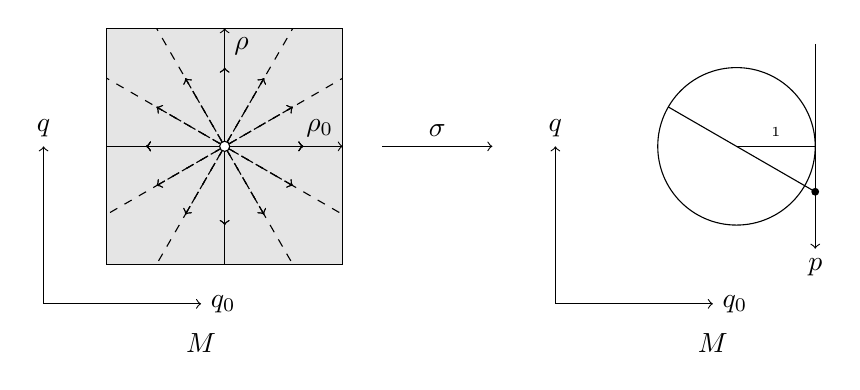
\begin{tikzpicture}
    \draw[->] (0, 0) -- (2, 0) node[anchor=west] {$q_0$};
    \draw[->] (0, 0) -- (0, 2) node[anchor=south] {$q$};
    
    \node (m) at (2.3, 2) {};
    
    \filldraw[draw=black, fill=gray!20] (m) ++(-1.5, -1.5) -- ++(0, 3) -- ++(3, 0) -- ++(0,-3) -- cycle;
    \draw[->] (m) ++(-1.5, 0) -- ++(3, 0) node[anchor=south east] {$\rho_0$};
    \draw[->] (m) ++(0, -1.5) -- ++(0, 3) node[anchor=north west] {$\rho$};
        
    \begin{scope}
        \clip (m) ++(-1.5,-1.5) rectangle ++(3, 3);
        \foreach \i in {0,30,...,180}{
            \draw[<->, dashed] (m) ++({-cos(\i)}, {-sin(\i)}) -- ++({2*cos(\i)}, {2*sin(\i)});
        }
        \foreach \i in {0,30,...,180}{
            \draw[<->, dashed] (m) ++({-cos(\i)}, {-sin(\i)}) -- ++({2*cos(\i)}, {2*sin(\i)});
        }
        \foreach \i in {0,30,...,180}{
            \draw[dashed] (m) ++({-4*cos(\i)}, {-4*sin(\i)}) -- ++({8*cos(\i)}, {8*sin(\i)});
        }
    \end{scope}
    
    \node[circle,draw=black,fill=white,inner sep=1.3pt] at (m) {};
    
    \draw[->] (6.5, 0) -- (8.5, 0) node[anchor=west] {$q_0$};
    \draw[->] (6.5, 0) -- (6.5, 2) node[anchor=south] {$q$};
    
    \node[fill=none] (m2) at (8.8, 2) {};
    
    \draw (m2) circle (1);
    \draw[->] (m2) ++(1, 1.3) -- ++(0, -2.6) node[anchor=north] {$p$} ;
    \draw (m2.center) ++(-0.866, 0.5) -- (9.8, 1.423) node[circle,fill=black, inner sep = 1pt] {};
    \draw (m2.center) -- ++(1, 0) node[pos=0.5,anchor=south] {\tiny{1}};
    %\draw[->] (m) ++(-1.5, 0) -- ++(3, 0) node[anchor=west] {$\rho_0$};
    %\draw[->] (m) ++(0, -1.5) -- ++(0, 3) node[anchor=south] {$\rho$};
    
    \draw[->] (4.3, 2) -- (5.7, 2) node[pos=0.5,anchor=south] {$\sigma$};
     
    \node at (2, -0.5) {$\ctzbundle{M}$};
    \node at (8.5, -0.5) {$\pctbundle{M}$};
\end{tikzpicture}

    \caption{Illustration of the principal $\mgroup$-bundle $\bundle{\ctzbundle{M}}{\pi}{\pctbundle{M}}$. The total space $\ctzbundle{M}$ is the cotangent bundle to $M$ with zero section removed, which is shown on the left. The action by the multiplicative group $\mgroup$ is illustrated by the arrows, for it acts as a scaling (dilation) on all the cotangent variables. The origin is not part of the fiber, for it is part of the zero section. The bundle projection $\pi$ projects all points that are on the same orbit (straight lines through the origin) to a single point on the base manifold: the projectivized cotangent bundle $\pctbundle{M}$. The former space has a symplectic structure while the latter space has a contact structure. Observe from \cref{eq:homo_coords} that $p = \rho/\rho_0$, i.e. such that $p$ is a coordinate for the projectivization by stereographic projection, as shown on the right.}
    \label{fig:principal_bundle}
\end{figure}

Define the \mgroup-\emph{action} $\raction{}$ on $\ctzbundle{M}$ as:
$$ \raction: \ctzbundle{M}\times\mgroup \to \ctzbundle{M} : \quad (q_0, q, \rho_0, \rho) \blacktriangleleft \lambda = (q_0, q, \lambda \rho_0, \lambda \rho ) \qquad \lambda \in \mgroup,$$
which are referred to as dilations of the fiber.

As illustrated in \cref{fig:principal_bundle}, the \emph{orbit space} of $\ctzbundle{M}$ with respect to the group action $\raction{}$ is the space of all points in $\ctzbundle{M}$ with all points on the same line through the origin (in the fiber) identified. This space is precisely equal to the projectivization of the cotangent bundle $\pctbundle{M}$. Hence, consider the \emph{principal} $\mgroup$-bundle $\bundle{\ctzbundle{M}}{\sigma}{\pctbundle{M}}$
\begin{center}
    \begin{tikzcd}
        \ctzbundle{M} \\ \ctzbundle{M} \arrow[u, "\raction{\mgroup}"] \arrow[d, "\sigma"] \\ \pctbundle{M} \cong \cbundle{M}
    \end{tikzcd}
\end{center}
The removal of the zero section is required for the group action to be free. The principal bundle $\bundle{\ctzbundle{M}}{\pi}{\pctbundle{M}}$ admits a \emph{fibered symplectic Liouville structure}, given by the Liouville form \cite{Libermann1987}
$$ \theta = \rho_0\dd{q_0} + \rho\dd{q}, $$
and the associated two-form $\omega = -\dd{\theta}$. The distinctive feature of these forms that makes this a Liouville structure is that they both commute with the group action $\raction{}$: \cite{Libermann1987}
$$ (\raction{\lambda})^* \theta = \lambda \theta \qquad \lambda \in \real_*,$$
which makes them homogeneous forms of degree 1.

The projection map $\sigma$ of the principal bundle is locally defined as 
\begin{equation}
    \sigma : \ctzbundle{M} \to \pctbundle{M}: (q_0, q, \rho_0, \rho) \mapsto (q_0, q, -\rho/\rho_0), 
    \label{eq:principal_projection}
\end{equation}
with $p \equiv -\rho/\rho_0$ a coordinate for the projectivized fiber. This coordinate does not cover the entire fiber: the points for which $\rho_0 = 0$ is missing (in \cref{fig:principal_bundle}, this point is the only point on the circle that cannot be projected on the $p$-axis). However, we will make the deliberate assumption that in our application, $\rho_0$ is never equal to zero.
%The manifold $\ctzbundle{M}$ is called the symplectization of the contact manifold. For now, we have not assigned any specific meaning to the coordinates given above, but they will turn out to match with the notation used in \cref{eq:lag_CK,eq:ham_CK}, etc.

Finally, the \emph{Liouville vector field} $Z$ associated with the Liouville structure is the vector field that represents the dilation of the fiber in the symplectization. It is defined as
\begin{equation}
    Z = \fromDual{\omega}(\theta) = \rho_0\pdv{}{\rho_0} + \rho\pdv{}{\rho}. 
    \label{eq:liouville_vf}
\end{equation}
Vector field (components) colinear with the Liouville vector fields are called \emph{vertical}; they represent dissipative action in the system. After the vertical components are removed, they remaining vector field is called \emph{horizontal}.

[Liouville automorphisms, commute with the Liouville vector field -> very important in the chapter about split-quaternions]

To summarize, we lifted the original system with symplectic structure $\wedgep{\dd{q}}{\dd{p}}$ to a contact manifold through the addition of a gauge variable $q_0$. We then symplectified the contact manifold to a four-dimensional system, with `positions' $(q_0, q)$ and `momenta' $(\rho_0, \rho)$.

\subsubsection{Homogeneous Hamiltonian systems} The theoretical construction of the past section serves an important purpose, because it is the symplectified space which is the proper setting for the Caldirola-Kanai Hamiltonian discussed in \cref{ssec:caldirola}. Along with the symplectification of the contact structure described in the past section, we can do the same with a contact Hamiltonian system.

There is a one-to-one correspondence between contact Hamiltonians on $\pctbundle{M}$ and a special class of Hamiltonians on the symplectified space $\ctzbundle{M}$. These are the Hamiltonians which are \emph{homogeneous} in the cotangent variables with degree 1:\footnote
{This is a consequence of the Euler theorem for homogeneous functions. If $\mathscr{H} = \mathscr{H}(\vec{q}, \vec{\rho})$ is homogeneous of degree $r$ in $\vec{\rho}$, then
    $$ \sum_{i = 1}^n \rho_i \pdv{\mathscr{H}}{\rho_i} = r \mathscr{H}. $$
 Therefore, for homogeneity of degree 1, we have: 
 $$ \lied{Z}{\mathscr{H}} = Z(\mathscr{H}) = \sum_{i=1}^n \rho_i \pdv{\mathscr{H}}{\rho_i} = \mathscr{H} \quad \text{with}\quad Z \equiv \sum \rho_i \pdv{}{\rho_i}. $$
 The correspondence between the 
}
\begin{equation}
    \mathscr{H}(q_0, q, \lambda \rho_0, \lambda \rho) = \lambda\,\mathscr{H}(q_0, q, \rho_0, \rho) \quad \text{or} \quad \lied{Z}{\mathscr{H}} = \mathscr{H},
\end{equation}
with $\lambda \in \real_0,\: H \in \functions{\ctzbundle{M}}$ and $Z$ defined according to \cref{eq:liouville_vf}. Given that $H$ is indeed homogeneous of degree 1, this correspondence is in canonical coordinates:
\begin{equation}
    \mathscr{H}(q_0, q, \rho_0, \rho) = -\rho_0\,H\qty(q_0, q, -\frac{\rho}{\rho_0})
    \label{eq:H_correspondence}
\end{equation}
where $\mathscr{H} \in \functions{\ctzbundle{M}}$, $H \in \functions{\pctbundle{M}}$ and $p = -\rho / \rho_0$ is a coordinate for the projectivized fiber. Likewise, there is also a direct correspondence between the vector fields generated by these Hamiltonians, and therefore the system dynamics. This is the reason why we go through the trouble of symplectification in the first place, it offers significant computational advantages. It is possible to derive the contact equations directly (as \citet{Bravetti2017} does), but it does not offer the same amount of insight as its symplectified counterpart. \cite{VanderSchaft2021a,Arnold1989}

Now, recall the Caldirola-Kanai Hamiltonian in \cref{eq:ham_CK}. Instead of assuming a direct time-dependence, we will think of the time-dependence as the gauge momentum, i.e. $\rho_0 \:``=" -\ec^{\gamma t}$. However, we will now consider $\rho_0$ to be a coordinate in its own right, instead of directly using the expression above --- the equality sign must therefore not be taken too literally. The Caldirola-Kanai Hamiltonian is then written as (cf. \cref{eq:ham_CK}):
$$ -\rho_0 \qty[\frac{1}{2m}\qty(-\frac{\rho}{\rho_0})^2 + \frac{1}{2}kq^2]. $$
The motivation to make this particular choice is twofold: first, observe that $\mathscr{H}$ is homogeneous in the cotangent variables $\rho_0, \rho$, and second, that their fraction yields the \emph{real} momentum: $ p = -\rho/\rho_0 $. However, we must acknowledge a potential dependence on $q_0$, since we want to convert the explicitly time-dependent Hamiltonian into a contact Hamiltonian. We therefore add the arbitrary function $f = f(q_0)$, whose value is to be determined later, and also multiply by $\rho_0$ to maintain homogeneity. The homogeneous Hamiltonian $\mathscr{H}$ is then:
\begin{equation}
    \mathscr{H}: \ctzbundle{M} \to \real: \quad \mathscr{H}(q_0, q, \rho_0, \rho) = -\rho_0 \qty[\frac{1}{2m}\qty(-\frac{\rho}{\rho_0})^2 + \frac{1}{2}kq^2 + f(q_0)]. 
    \label{eq:homo_hck}
\end{equation}
 Using the correspondence given by \cref{eq:H_correspondence}, the homogeneous Hamiltonian may be `projected' to the contact Hamiltonian $H$:
\begin{equation}
    H: \pctbundle{M} \to \real: \quad H(q_0, q, p) = \frac{p^2}{2m} + \frac{1}{2}kq^2 + f(q_0).
\end{equation}
Numerically, this contact Hamiltonian is the same as the Hamiltonian for an undamped mass-spring system but it is defined on the contact manifold that also takes into account the gauge variable $q_0$.

\paragraph{Equations of motion} Now to derive the equations of motion. As mentioned, this is easiest in the symplectified space because Hamilton's equations can be readily applied (the reader can consult \cref{app:contact_geometry} for the direct derivation). Because we are using canonical coordinates, the Hamiltonian vector field
\begin{equation}
    X_\mathscr{H} = \fromDual{\omega}(\dd{\mathscr{H}})
    \label{eq:ham_vf}
\end{equation}
corresponds to Hamilton's equations in the familiar form:
\begin{equation}
    \dv{\rho}{t} = -\pdv{\mathscr{H}}{q},\quad
        \dv{\rho_0}{t} = -\pdv{\mathscr{H}}{q_0},\quad
        \dv{q}{t} = \pdv{\mathscr{H}}{\rho},\quad
        \dv{q_0}{t} = \pdv{\mathscr{H}}{\rho_0}.
\end{equation}
Observe that this motivates why one has to take the partial with respect to the `other' momentum in the Caldirola-Kanai momentum: we are dealing with a specific instance of a more general class of homogeneous coordinates of the cotangent variables. Of course, the variable of interest is the actual momentum $p$, not the scaled version $\rho$. The time-derivative of $p$ can be written in terms of $\rho$ and $\rho_0$, completely analogous to \cref{eq:momentum_relation}:
\begin{equation}
    p = -\rho/\rho_0 \quad\Rightarrow\quad \dv{p}{t} = -\frac{1}{\rho_0}\dv{\rho}{t} + \frac{\rho}{\rho_0^2}\dv{\rho_0}{t} = -\frac{1}{\rho_0}\dv{\rho}{t} - \frac{p}{\rho_0}\dv{\rho_0}{t}. 
    \label{eq:homo_momenta}
\end{equation}
Given \cref{eq:homo_hck}, the partial derivatives of $\mathscr{H}$ and $H$ are related through the by relations: \cite{Arnold1989}
\begin{equation}
    \begin{split}
        \pdv{\mathscr{H}}{q} &= -\rho_0 \pdv{H}{q}, \\
        \pdv{\mathscr{H}}{q_0} &= -\rho_0 \pdv{H}{q_0}, \\
        \pdv{\mathscr{H}}{\rho} &= -\rho_0 \pdv{H}{p}\pdv{p}{\rho} = \pdv{H}{p}, \\
        \pdv{\mathscr{H}}{\rho_0} &= -H - \rho_0 \pdv{H}{p}\pdv{p}{\rho_0} = -H - \pdv{H}{p}\frac{\rho}{\rho_0} = \pdv{H}{p}p - H.\\
    \end{split}
    \label{eq:partial_relation}
\end{equation}
Hence, the \emph{contact} equations of motion can be found by combining of \cref{eq:momentum_relation} and \cref{eq:partial_relation}:
\begin{equation}
    \begin{split}
        \dv{q}{t} &= \pdv{H}{p} \\
        \dv{p}{t} &= \frac{1}{\rho_0}\pdv{\mathscr{H}}{q} + \frac{p}{\rho_0}\pdv{\mathscr{H}}{q_0} = - \pdv{H}{q} - p\pdv{H}{q_0} \\
        \dv{q_0}{t} &= \pdv{H}{p}p - H.
    \end{split}
    \label{eq:contact_eom}
\end{equation}
Some observations are important to note:
\begin{itemize}
    \item The evolution of the position $q$ remains the same as for the `normal' (undamped) case.
    \item The evolution of the momentum operator picks up a term that is depends on presence of the gauge variable in the contact Hamiltonian.
    \item The evolution of the gauge variable is equal to the Legendre transformation of the contact Hamiltonian with respect to $p$.
\end{itemize}

We are now ready to determine the nature of the as of yet unknown function $f$ to obtain the correct equations of motion. By comparing \cref{eq:homo_momenta} and \cref{eq:contact_eom}, the following relation must hold:
$$ \frac{1}{\rho_0}\dv{\rho_0}{t} = \pdv{H}{q_0} = \dv{f}{q_0}. $$
Furthermore, since we initial `substituted' $\ec^{\gamma t}$ in favor of $\rho_0$, the left hand side of the equation should be equal to $\gamma$ for it to be consistent with the Caldirola-Kanai Hamiltonian. Hence, we know that $\dv{f}{q_0} = \gamma$, or $f(q_0) = \gamma q_0$ up to a constant, which we choose to be zero. Although this may seem like an odd construction, the only thing we did is made the contact equation of motions equivalent with the time-dependent equations of motion. Now, the fact that $\rho_0 = \ec^{\gamma t}$, ceases to be an a priori assumption, and is derivable through Hamilton's equations:
$$ \dv{\rho_0}{t} = -\pdv{\mathscr{H}}{q_0} = \gamma\rho_0 \quad \Rightarrow \quad \rho_0 = \ec^{\gamma t} + C$$

As such, we have for the contact Hamiltonian:
\begin{equation}
    H: \pctbundle{M} \to \real: \quad H(q_0, q, p) = \frac{p^2}{2m} + \frac{1}{2}kq^2 + \gamma q_0,
    \label{eq:H_dho}
\end{equation}
and this is precisely Bravetti's result. For the homogenous Hamiltonian on the symplectified space, we have:
\begin{equation}
    \mathscr{H}: \ctzbundle{M} \to \real: \quad \mathscr{H}(q_0, q, \rho_0, \rho) = -\rho_0\,\qty[\frac{1}{2m}\qty(-\frac{\rho}{\rho_0})^2 + \frac{1}{2}kq^2 + \gamma q_0]. 
    \label{eq:H_dho_homo}
\end{equation}
%It is easily verified that the contact Hamilton equations $\cref{eq:contact_eom}$ yield the correct equations of motion for the damped harmonic oscillator:
%$$ \dv{q}{t} = p/m \qquad \dv{p}{t} = -kq -\gamma p.$$
%On the other hand, the equation of motion for $q_0$ requires some additional considerations; this is the subject of the next section.

The Hamiltonian vector field $X_\mathscr{H} \in \vfields{\ctzbundle{M}}$ is then, using \cref{eq:H_dho_homo} and \cref{eq:ham_vf}:
$$ X_{\mathscr{H}} = -\frac{1}{m}\frac{\rho}{\rho_0}\pdv{}{q}\: + \: \qty[\frac{1}{2m}\qty(\frac{\rho}{\rho_0})^2 - \frac{1}{2}kq^2 - \gamma q_0]\pdv{}{q_0}\: + \: \rho_0 kq \pdv{}{\rho}\: + \: \gamma \rho_0 \pdv{}{\rho_0}.$$ 

The contact Hamiltonian vector field $X_H \in \vfields{\pctbundle{M}}$ is obtained either by using the contact Hamilton equations given by \cref{eq:contact_eom}, or by using the pushforward of the projection map $\sigma$:
$$ X_H = \sigma_*\,X_\mathscr{H} = \frac{p}{m}\pdv{}{q}\: + \: \qty(\frac{p^2}{2m} - \frac{1}{2}kq^2 - \gamma q_0)\pdv{}{q_0}\: - \: (kq + \gamma p)\pdv{}{p}\: $$
This is essentially the equivalent of the time-dependent transformation performed in \cref{ssec:caldirola}. Clearly, these yield the correct equations of motion for the damped harmonic oscillator.

\paragraph{Mechanical energy} One of the computational advantages of the symplectified space is the fact that `regular' Poisson brackets can be used in contrast to their slightly unwieldy contact counterparts.\footnote
{The Poisson bracket is defined as 
    $$ \poisson{f}{g} = \omega(X_f, X_g) = \lied{X_g}{f},$$
 where $X_f$ and $X_g$ are the Hamiltonian vector fields of $f$ and $g$. \cite{Libermann1987}
} 
The mechanical energy, denoted by $E$, is equal to 
$$ E: \pctbundle{M} \to \real: \quad E(q_0, q, p) = \frac{p^2}{2m} + \frac{1}{2}kq^2,$$
With some abuse of notation, we will denote both functions on the contact space and their lifted version to the symplectified space by the same symbol. That is to say, the function $E$ both refers to $E \in \functions{\pctbundle{M}}$ and $(E \circ \sigma) \in \functions{\ctzbundle}$.

The change of mechanical energy in the system is then readily determined using the Poisson brackets:
$$ \dv{E}{t} = \poisson{E}{\mathscr{H}} = \lied{X_\mathscr{H}}{E} = -\frac{\gamma}{2m}\qty(\frac{\rho}{\rho_0})^2 = -\frac{\gamma}{2m}p^2,$$
which is precisely the dissipative power in the damping element.

\todo{Check minus signs of the change in mechanical energy, should be opposite to heat generated.}
\todo{Finish Poincaré lemma discussion.}

\begin{mathbox}{The importance of the zero section}
    It may be tempting to disregard the removal of the zero section from the cotangent bundle as a mathematical technicality. It has, however, deep implications for the nature of the Hamiltonian systems that can be defined on it, encoded in the so-called de Rham cohomology groups.
    
    Suppose that $Y$ is a symplectic vector field with $\omega$ the symplectic form. The 1-form
    $$\xi = \intpr{Y}{\omega}$$
    is necessarily closed, because
    $$ \dd{\intpr{Y}{\omega}} \; = \underbrace{\bcancel{\lied{Y}{\omega}}}_{Y \text{ symp.}}\;- \; \underbrace{\bcancel{\intpr{Y}{\dd{\omega}}}}_{\omega \text{ closed}}\; = 0. $$
    The Poincaré lemma (a specific instance of the de Rham cohomology) says that on a \emph{contractible domain}, all closed forms are necessarily also exact (the converse is true on any manifold, for $\dd{}^2 = 0$). This would mean that, if $\xi$ were to be defined on a contractible manifold, it would automatically be an exact form (this is the same as saying that on these types of manifolds, all symplectic vector fields are Hamiltonian). In other words, there must be a function $\mathscr{H}$ such that $\xi = \dd{\mathscr{H}}$.

    Integration around curve to show that $\xi$ in our case is not exact. Hard, because over two charts.

    Also show that the region of interest is not simply connected in order to use de Rham in the first place.
    $ \real^4 / \{(q_0, q, 0, 0)\} $ not simply connected
\end{mathbox}

\subsubsection{Physical interpretation of the gauge variables}
Another advantage of using the purely symplectic formalism on the lifted space is the fact that the homogeneous Hamiltonian is invariant under the flow it generates, since the explicit time-dependence has been removed:
$$ \dv{\mathscr{H}}{t} = \poisson{\mathscr{H}}{\mathscr{H}} = \lied{X_{\mathscr{H}}}{\mathscr{H}} = 0. $$
We may therefore associate the homogeneous Hamiltonian with a constant. By inspection of \cref{eq:H_correspondence}, 
$$ \mathscr{H}(q_0, q, \rho_0, \rho) = -\rho_0\,\underbrace{\qty(C\rho_0^{-1})}_{H} \qquad C \in \real.$$
Recall that we made the assumption earlier that $\rho_0$ is a function \emph{without zeros}. 

The constant $C$ is a degree of freedom in the system that we are free to choose, for the equations of motion will be consistent with any chosen value. This called a \emph{gauge} of the system, and its choice will influence the value of the gauge variable directly. The contact Hamiltonian is not a constant of motion however (at least, for dissipative systems). With some abuse of notation
$$ \dv{H}{t} = C\,\dv{\rho_0}{t}  = -C\,\pdv{\mathscr{H}}{q_0}.$$
Until now, there were no assumptions regarding the value of the damping constant $\gamma$: indeed, the `normal' equations of motion are readily derived when $\gamma$ is set to zero. We will now add the assumption that there is at least some dissipation present in the system ($\gamma \neq 0$) to assign further intrepretation to the gauge variable. The evolution of $q_0$ is directly related to the evolution of $H$ by \cref{eq:H_dho}
$$ 
    q_0 = \frac{1}{\gamma} \bigg(\rho_0 C - \underbrace{\frac{p^2}{2m} - \frac{1}{2}kq^2}_{E}\bigg)
$$
Because we are free to choose the value of $C$, let us now make a choice of particular interest; namely $C = 0$. In that case, both $\mathscr{H}$ and $H$ vanish \emph{weakly};\footnote
{The weak equality, as opposed to the strong equality, is not maintained under variations. Hence, although the numerical value of the function is zero, its partial derivatives do not necessarily vanish. The reader is referred to \citet{Dirac1950} for a more elaborate discussion.}
this choice rids us from the additional freedom in $C$ that would also show up in the equation of motion for $q_0$. Instead, $q_0 = - E/\gamma$; which can be interpreted as the heat dissipated by the system (one can add a suitable initial condition for $q_0(0) = E(0)$ to make this also numerically correct). This `heat' function will be called $Q$; we therefore have
$$ q_0 = Q/\gamma. $$
The vanishing of the Hamiltonians reflects the energy balance that is maintained throughout the evolution of the system:
\begin{equation*}
    \begin{split}
        H &= E + Q \\
          &= \text{\textsc{mechanical energy}} + \text{\textsc{dissipated heat}}.
    \end{split}
\end{equation*}
The fact that $H$ vanishes makes it a constant of motion on par with the symplectified Hamiltonian $\mathscr{H}$. This careful choice of for the gauge variable removes a lot of the ambiguity that is naturally present in contact systems; this rather subtle point is a bit overlooked by past research. \cite{Bravetti2017} 
Furthermore, the evolution of the dissipated heat is
$$ \dv{Q}{t} = \gamma \dv{q_0}{t} = \gamma \qty[\frac{1}{2m}\qty(\frac{\rho}{\rho_0})^2 - \frac{1}{2}kq^2 - \gamma q_0] = \gamma\frac{1}{2m}\qty(\frac{\rho}{\rho_0})^2, $$
which is the expected result.

This very particular choice for the gauge variable may seem a little arbitrary. However, \emph{in general}, the time-rate of change
$$
    \jacobi{f}{g}
$$

\todo{Canonical transformation}
\todo{Action-angle coordinates}
\todo{Generalization using Jacobi problems}



%% LAGRANGIAN SYSTEM
\section{Contact Lagrangian systems}
\label{sec:lagrangian}
In the classic, symplectic case, the Legendre transformation is used to pass from the Hamiltonian to the Lagrangian formalism and vice versa. This is because the Legendre transform facilitates a mapping between the tangent and cotangent bundle. If the Lagrangian (or Hamiltonian) is (hyper)regular (i.e. the mass matrix is invertible), this mapping is a diffeomorphism. \cite{Carinena1990}

One would be tempted to use the normal Legendre transformation on the symplectified Hamiltonian $\mathscr{H}$. This approach will meet some problems though:
\begin{itemize}
    \item A homogeneous function is not regular in the homogeneous variables --- naturally, a degree of freedom still resides in the action of the multiplicative group. Therefore, the mapping from the cotangent to the tangent bundle is not a diffeomorphism. Said otherwise, there is not a one-to-one correspondence between the homogeneous momenta and the associated velocities in the Lagrangian description.
    \item As a consequence of Euler's theorem for homogeneous functions, the Legendre transformation for a homogeneous function is necessarily equal to zero. For any homogeneous function $H$ (of degree 1), Euler's theorem states that
    $$ \sum_{i = 1}^n \rho_i \pdv{\mathscr{H}}{\rho_i} = \mathscr{H}, $$

        i.e. the function is equal to its associated `action', and therefore the expression for the Legendre transformation vanishes. \cite{Dirac1950,Dirac1933}
\end{itemize}
There is a better path to take. In essence the Legendre transform is (and was originally meant to be) a \emph{contact transformation}.

\section{Generalization to other mechanical systems}
\label{sec:generalization}


